
\chapter{初期グラフによる探索空間の削減}
\label{chap:reduce-by-initial-graph}
\ref{sect:apply-to-gmg}節で述べた初期グラフを変更することで,
探索空間を削減できる.本章では,いくつかの初期グラフを与え,その効果を
実験により検証する.

\section{長さ$2Q+2$の閉路をもつ初期グラフ}
\label{sect:initial-graph-cycle}
\begin{example}
  前述の手順に従って構築した,頂点数12,次数3の初期グラフを
  図\ref{fig:initial-graph-cycle-example}に示す.
  \begin{figure}
    \centering
    \includegraphics[width=.5\linewidth]{initial-tree-cycle-example.pdf}
    \caption{長さ6の閉路を含む,頂点数12,次数3の初期グラフ}
    \label{fig:initial-graph-cycle-example}
  \end{figure}
\end{example}

\section{全域木}
\label{sect:initial-spanning-tree}
\begin{conjecture}[全域木予想]
  \label{conj:spanning-tree}
  一般化ムーアグラフの誘導グラフには,次のような全域木が存在する.
\end{conjecture}
\begin{example}
  予想\ref{conj:spanning-tree}に従っていくつかの全域木を構築する.
  構築した初期グラフを図\ref{fig:initial-spanning-tree-example}に示す.
  \begin{figure}
    \centering
    \subfloat[頂点数$12$,次数$3$の全域木]{
      \includegraphics[width=.4\linewidth]
                      {initial-spanning-tree-12-example.pdf}
    }\hfill
    \subfloat[頂点数$18$,次数$3$の全域木]{
      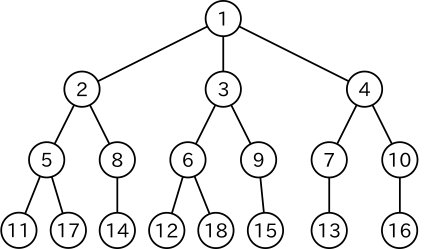
\includegraphics[width=.45\linewidth]
                      {initial-spanning-tree-18-example.pdf}
    }
    \caption{全域木の例}
    \label{fig:initial-spanning-tree-example}
  \end{figure}
\end{example}

\section{実験}
\label{sect:exp-reduce-by-initial}

\section{結果}
\label{sect:result-reduce-by-initial}
